%---------------------------------------------------------------------
%   documentclass
%---------------------------------------------------------------------
\documentclass[a4paper]{article}

%---------------------------------------------------------------------
%   packages
%---------------------------------------------------------------------
\usepackage{mathtools}
\usepackage[english]{babel}
\usepackage[enc=cp1250]{hrlatex}
\usepackage[T1]{fontenc} %pekne makcene
\usepackage{lmodern} %spolu s T1 smooth font!
\usepackage{hyperref} %odkazy
\usepackage{amsmath}
\usepackage{amsthm}
\usepackage{cite} %bibtex
\usepackage{enumitem}
\usepackage{titlesec} %section titles font size change
\usepackage{color} %for \definecolor
\usepackage{colortbl} %for \rowcolor command
\usepackage{eucal} %for nice letters like \mathcal{A}
\usepackage{tikz}
\usepackage{scalefnt}
\usepackage{booktabs}% http://ctan.org/pkg/booktabs
\usepackage{multirow}% http://ctan.org/pkg/multirow
\usepackage{pifont} %for ticks (check symbols)
\usepackage{listings}
\usepackage{floatflt} %to have tables and text beside
\usepackage{courier}
\usepackage{subcaption}

%---------------------------------------------------------------------
%   margins
%---------------------------------------------------------------------
\oddsidemargin 0.0in
\evensidemargin 0.0in
\textwidth 6.1in
\textheight 23.94cm
\topmargin -0.35in

%---------------------------------------------------------------------
%   various settings
%---------------------------------------------------------------------
\pgfrealjobname{r-12-12-20} % <-- NOTE: this needs to be the real document's basename
                        %     (else you'll only get an empty output file)

\newif\ifmine % introduce a switch for draft vs. final document
\minetrue

\newif\iffinal % introduce a switch for draft vs. final document
\finaltrue % use this to compile the final document
\iffinal
  \newcommand{\inputTikZ}[1]{%
    \input{#1.tikz}%
  }
\else
  \newcommand{\inputTikZ}[1]{%
    \beginpgfgraphicnamed{#1-external}%
    \input{#1.tikz}%
    \endpgfgraphicnamed%
  }
\fi

\setlist{nolistsep} %so that lists have normal spacing

\titleformat{\section}{\LARGE\bfseries}{\thesection}{1em}{} %section titles
\titleformat{\subsection}{\Large\bfseries}{\thesubsection}{1em}{} %subsection titles

\definecolor{tablehead}{RGB}{238,233,233} %nice smooth grey

\setlength{\parindent}{0pt} %we don't need no indentation

\graphicspath{{./pics/}} %picture dir

\definecolor{lstcolor}{RGB}{238,233,233}

\lstset{ %
    language=Octave,                % choose the language of the code
    basicstyle=\footnotesize\ttfamily,       % the size of the fonts that are used for the code
    numbers=left,                   % where to put the line-numbers
    numberstyle=\footnotesize,      % the size of the fonts that are used for the line-numbers
    stepnumber=1,                   % the step between two line-numbers. If it's 1 each line will be numbered
    numbersep=5pt,                  % how far the line-numbers are from the code
    backgroundcolor=\color{lstcolor},   % choose the background color. You must add \usepackage{color}
    showspaces=false,               % show spaces adding particular underscores
    showstringspaces=false,         % underline spaces within strings
    showtabs=false,                 % show tabs within strings adding particular underscores
    frame=single,	                % adds a frame around the code
    tabsize=2,	                    % sets default tabsize to 2 spaces
    captionpos=b,                   % sets the caption-position to bottom
    breaklines=true,                % sets automatic line breaking
    breakatwhitespace=false,        % sets if automatic breaks should only happen at whitespace
    title=\lstname,                 % show the filename of files included with \lstinputlisting; also try caption instead of title
    escapeinside={\%*}{*)},          % if you want to add a comment within your code
%    morekeywords={*,...}            % if you want to add more keywords to the set
	deletekeywords={all, null, length, path, function}
}

%---------------------------------------------------------------------
%   environments
%---------------------------------------------------------------------
\renewenvironment{abstract}[1]
{
	\Large
	\begin{center}
		\textbf{#1}
	\end{center}
	
	\normalsize
	
	\addtolength{\leftskip}{1in}
	\addtolength{\rightskip}{1in}
	\setlength{\parindent}{0in}
}
{
}

\newenvironment{itemizesp}
{
    \begin{itemize}
}
{
    \end{itemize}
}

\newcommand{\deftoken}{\boldmath{$\mathcal{DEFINITION}$}}
\newcommand{\restoken}{\boldmath{$\mathcal{RESULT}$}}
\newcommand{\dotoken}{\boldmath{$\mathcal{DO METHOD}$}}
\newcommand{\textbff}[1]{{\large \textbf{#1}}}
\newcommand{\tick}{\ding{52}}

\newtheorem{definition}{Definition}
\newtheorem{lemma}{Lemma}
\newtheorem{observation}{Observation}

%---------------------------------------------------------------------
%   magic code
%---------------------------------------------------------------------
% Here it is: the code that adjusts justification and spacing around caption.
\makeatletter
% http://www.texnik.de/floats/caption.phtml
% This does spacing around caption.
\setlength{\abovecaptionskip}{6pt}   % 0.5cm as an example
\setlength{\belowcaptionskip}{6pt}   % 0.5cm as an example
% This does justification (left) of caption.
\long\def\@makecaption#1#2{%
  \vskip\abovecaptionskip
  \sbox\@tempboxa{#1: #2}%
  \ifdim \wd\@tempboxa >\hsize
    #1: #2\par
  \else
    \global \@minipagefalse
    \hb@xt@\hsize{\box\@tempboxa\hfil}%
  \fi
  \vskip\belowcaptionskip}
\makeatother

%---------------------------------------------------------------------
%   document
%---------------------------------------------------------------------
\begin{document}
    \thispagestyle{empty}
    %---------------------------------------------------------------------
    %   topmatter
    %---------------------------------------------------------------------
    \title{\textbf{r-2012-12-20}}
    \author{Franti�ek Hajnovi� \\
    \texttt{ferohajnovic@gmail.com}}
    \date{\today}
    \maketitle

    \vskip 0.5cm

    %---------------------------------------------------------------------
    %   OUTLINE
    %---------------------------------------------------------------------
    \tableofcontents
    
	%---------------------------------------------------------------------
    %   Emergence of timetables    
    %---------------------------------------------------------------------        

\newif\ifbordel
\bordelfalse
\ifbordel

Timetables satisfy certain \textit{regularities}. For example, if a (direct) connection from $A$ to $B$ at \textit{12:00} takes one hour, it is unlikely that a different (direct) connection between $A$ and $B$ at another time would be much longer or shorter. We may specify these kind of regularities when building a timetable    

We will now shortly describe the characteristics of each type of timetable. \\
		
		\textbf{Regional buses}. \\
		
		\textbf{Country-wide rails}. \\
		
		\textbf{Underground rails}. \\
		\begin{itemize}
			\item Any intersection on a map of the underground is 
		\end{itemize}
		
		\textbf{Public transportation (buses)}. \\
		\begin{itemize}
			\item 
		\end{itemize}
		
		\textbf{Airlines}
		\begin{itemize}
			\item The graph of airport connections (an edge is between a pair of airports connected by at least one flight) has a scale-free distribution of degrees. We can take this for the underlying graph, though without any knowledge about the timetable, it would not be able to obtain the graph.
			\item Usually, planes fly between a given pair of cities back and forth with constant pause at each end (to refuel, load customers...). This results in a pendulum-like timetable with a (more or less) constant period for repeated connections.
		\end{itemize}
		
		%properties - HD, separator, scale-free-ness
		
		Assume we have an \textit{underlying weighted, oriented graph} (representing the transportation network). The weights will be e.g. the distance between nodes, or a similar metric. Meaning of a node varies - see table \ref{tab:networks} for the usual meaning. In the easiest setting when generating timetable on top of this graph we may assume, that \textit{each node of the underlying graph is a station}. This is clearly not a real scenario in many cases - e.g. there is not a bus stop on every intersection and many times the bus stop is actually \textit{between} intersections, i.e. on a road - e.g. there may be a long road with several bus stops spread over it. We will call this a \textbf{problem of long road} and the first problem, when stations are in too many nodes of the underlying graph will be called \textbf{station overfill}.
		
				In what follows, we will try to provide more and more accurate ways of creating a timetable. Accurate in a way, that it would more or less correspond to the real world timetables built on a corresponding transportation network. \\
		
		
		
		
		
		
		
		
		
\fi	
 
	\section{Emergence of timetables}
		\subsection*{Types of timetables and underlying networks}
		The purpose of this thesis is to investigate the properties of timetable graphs and to create distance (or rather earliest arrival) oracles that would take advantage of the good properties to efficiently answer EAP queries. One way to understand the properties of the timetables is to \textit{describe their creation}. \\
		
		The first thing we should notice when it comes to the creation of a timetable is that there is some sort of underlying transportation network - e.g. for buses it is the road network, for trains the rail network etc... \footnote{Exception may be the airline timetable which does not really exploit an existing transportation network. However, we may simulate the underlying transportation network as a complete graph with nodes being the airports.} This transportation network is being used by each connection, thus its properties should influence the properties of the timetable. Table \ref{tab:networks} summarises several different types of timetables and corresponding underlying transportation networks.  \\
		
		\begin{table}[h]{
			\scriptsize
		    \begin{tabular}{l|c}
			%legend
			\hline
				\rowcolor{tablehead}
	           	\textbf{Type of timetable} & 
	           	\textbf{Underlying network} \\
	        %data
	        \hline
	            Regional bus & road network \\
	            Country-wide rails & railway network \\
	            Underground rails & underground railways \\
	            Public transportation (buses) & road network (city)  \\
	            Airlines & none (complete graph on airports) \\
	        \end{tabular}}
			\caption{\label{tab:networks} Types of timetables and corresponding underlying transportation networks}
	        \normalsize
		\end{table}
		
		\textit{Note:} We would be able to find more types of timetables, each with at least slight differences with respect to the others. However, for our purposes, the mentioned five types are sufficient. \\		
		
		First thing to realize is that the \textbf{underlying transportation network} is something else then the \textbf{underlying graph} of a given timetable. The former is really a map of the infrastructure used by the carriers of the timetable (nodes are intersections, edges are roads/rails between them...) and the nodes do not have to be equivalent to stations of the timetable. The latter is an oriented graph with stations being the nodes and arcs specifying from where to where there can be an elementary connection. Thus generating timetables on top of the \textit{graph of the underlying network} is not the best approach. \\
		
		Let us take e.g. the road network - there are quite efficient algorithms to find shortest paths in road networks. Their functionality depends on several good properties of road networks. If we would like to show that these properties are present in the graphs representing e.g. regional bus timetables (which have road network as the underlying transportation network), we would have to show the preservation of the properties at two places: \\
		
		\begin{center}
			\textit{Underlying network} $\xrightarrow{a)}$ \textit{Underlying graph} $\xrightarrow{b)}$ \textit{Timetable}
		\end{center}
		
		You can think of this as of a game with two levels of difficulties. The more difficult version is the following: We have an underlying network of some timetable that we do not know. Our task is to choose stations on this network and then build a timetable connecting these stations so that it reflects the original timetable as much as possible. A bit easier version is the one, when we already know the stations and the pairs of stations between which there are elementary connections. \\
		
		So in the \textbf{step \textit{a)}} we first have to think where do we want to have stations and which of them should be connected in the timetable. The \textit{stations may be placed} in the nodes of the network, or on edges, in which case they cut the edge in two and create a new node. Then we \textit{specify the infrastructure} which is simply marking the arcs that will be used. Next, we \textit{remove} from the graph each \textit{node on which we have not placed a station}, and add new edges between each pair of its neighbours to preserve their connectivity and distance. And finally, we keep for each set of arcs from $X$ to $Y$ only the one with minimum length. After this, we have an underlying graph for a timetable with stations as we chose them and with elementary connections possible according to the arcs of the graph. See picture \ref{pic:stepa} for demonstration. \\
		
		\begin{figure}[h!]
			\begin{subfigure}{.33\textwidth}
  				\centering
				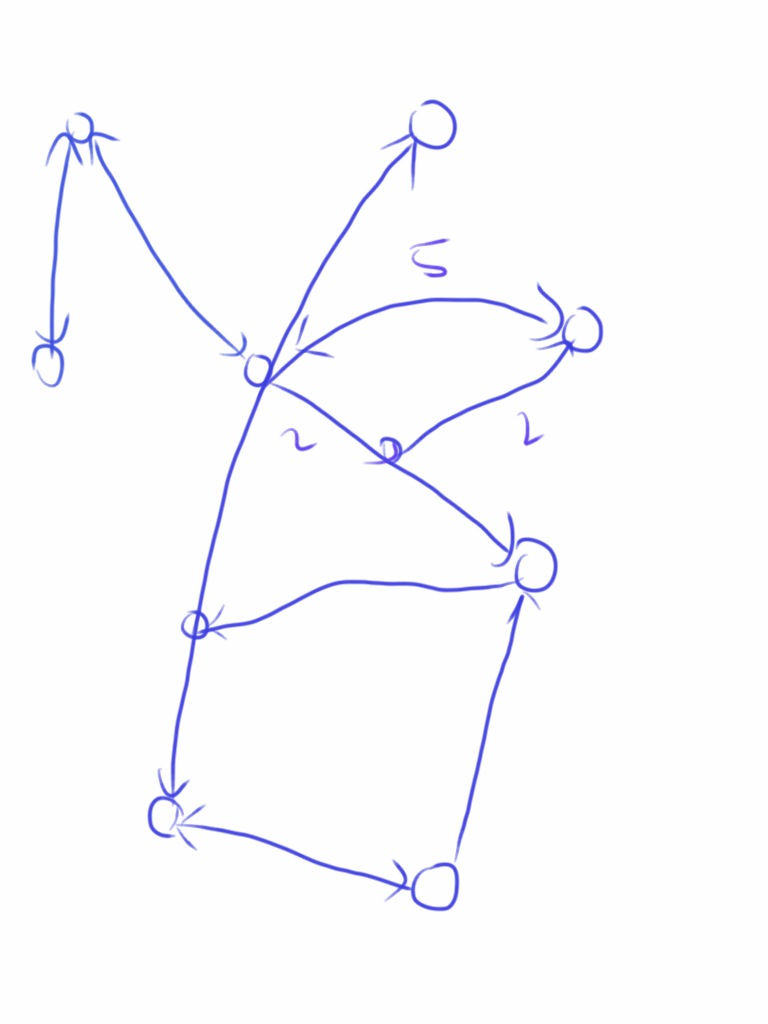
\includegraphics[width=1.2\linewidth]{stepa1.JPG}
	  			\caption{Underlying network}
	  			\label{pic:stepa1}
			\end{subfigure}%
			\begin{subfigure}{.33\textwidth}
  				\centering
				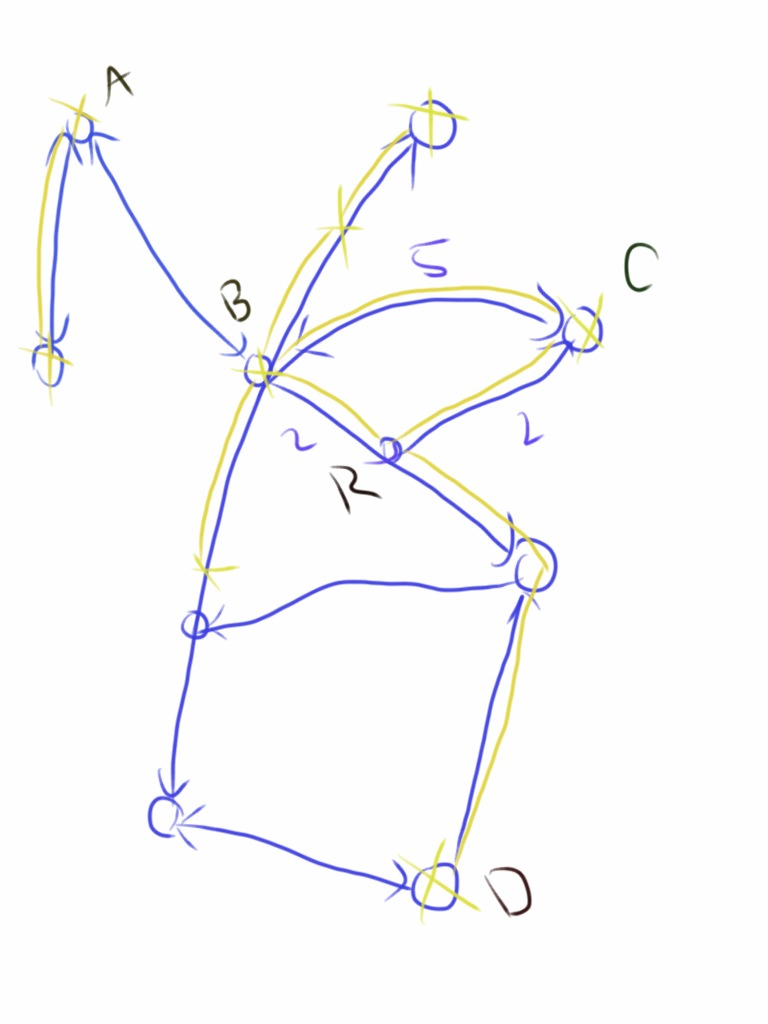
\includegraphics[width=1.2\linewidth]{stepa2.JPG}
	  			\caption{Chosen stations and infrastructure}
	  			\label{pic:stepa2}
			\end{subfigure}%
			\begin{subfigure}{.33\textwidth}
  				\centering
				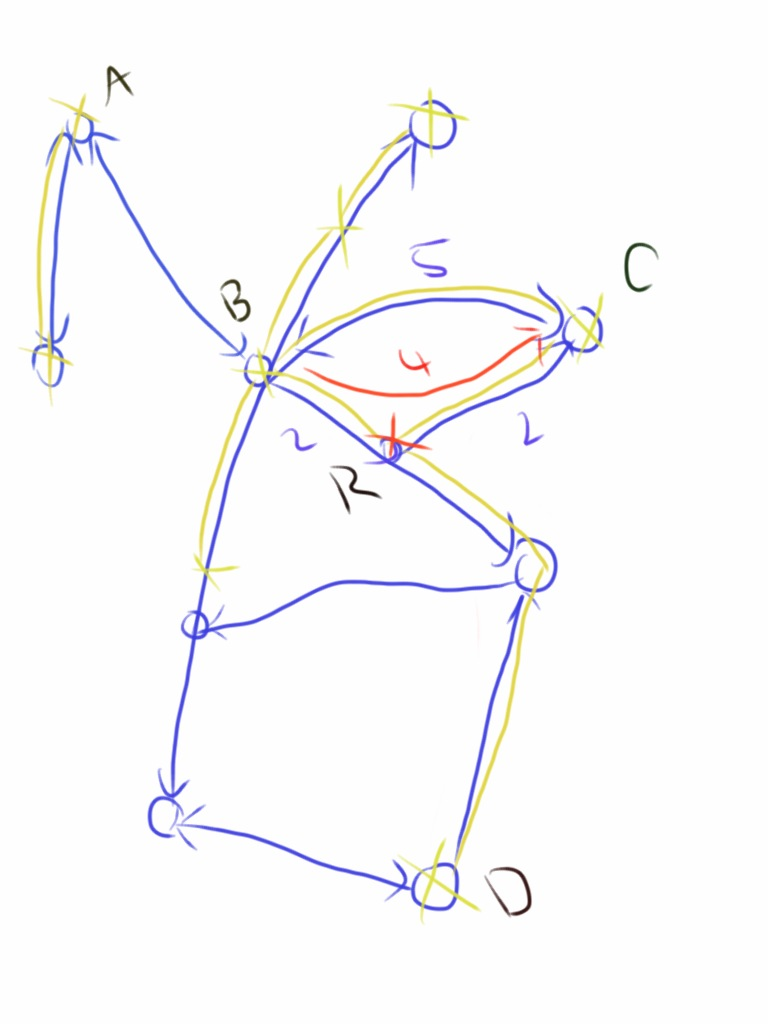
\includegraphics[width=1.2\linewidth]{stepa3.JPG}
	  			\caption{Removed non-station nodes}
	  			\label{pic:stepa3}
			\end{subfigure}%
			\caption{Step \textit{a)}. First we have the underlying transportation network \textit{(a)}. Then we choose the stations and infrastructure (marked yellow, \textit{(b)}). Note that there will be no connection between $A$ and $B$ in the timetable since they are not connected. Finally we remove node $R$, since it is a non-station node and we insert a new arc from $B$ to $C$ to preserve the distance \textit{(c)}. Similarly we would do between $B$ and $D$ and $C$ and $D$.}
	  		\label{pic:stepa}
        \end{figure}
        
        In the \textbf{step \textit{b)}}, we have to build a timetable respecting the locations of the stations and the connections between them. We will discuss this later. In what follows, we will be interested, if by restricted selection of stations and infrastructure, we can preserve the good properties through step \textit{a)} - that is from underlying network to the underlying graph. \\
        
		\subsection*{Step a) - discussion}
		A question is - how do we choose stations on the transportation networks? In a real-world scenarios, the placement of stations is simply determined by the necessity of transportation from a given place - thus there will most probably be many stations near (or in) the big cities, holiday resorts etc. Unless we have a geographic representation of the transportation network and we consult external source of information, we are unable to deduce the right placement of the stations. \\
		
		However, even the mere graphical representation of a transportation network provides some clues. E.g., if we see a \textbf{cluster of many nodes} connected by short roads, we most probably found a city (or another important place). The size of a cluster would be influenced by the size of the city, which is usually proportional to the number of stations found within. \\
		
		Another idea is to take nodes which form \textbf{separators} (or are part of small separators) in the network. These nodes are likely to be important as they connect different parts of the map and we could expect a station being built in such node, though a station of low importance (e.g. a station at the borders of two states, used for transfers). Note: a separating \textit{edge} is intuitively unlikely to carry a station, especially a longer edge, as it is usually connecting bigger components (e.g. a road in a desert between Las Vegas and Los Angeles) . \\
		
		We could also try to place stations based on the \textbf{betweenness centrality measure} of a node, which is equal to the number of shortest paths passing through the specific node. In cities, these are likely to be used as bus stations and generally, these nodes would be ideal for transit stations. \\			
		
		\subsection*{Step b) - discussion}
		As for the step \textit{b)}, there are numerous decisions that influence the properties of the resulting timetable. Let us list the most important ones:
		\begin{itemize}
			\item \textbf{Usage of express lines}. Express lines were defined in \textit{r-12-11-08} and if we allow them, we can add an elementary connection also between two stations \textit{not} connected by an edge in the underlying graph. However, we have to be careful about this, as excessive usage of express line could completely hide the structure of the underlying graph. One possibility is to assign levels to stations (a plausible option would be such that the distribution of the levels would be scale-free) and make express lines only between pairs of stations with the same level (or with a difference of $1$ in levels).
			\item \textbf{Specifying length of connections}. Here we could parametrize, how much do we hold on to the cost of the edges of the underlying graph. For example, if the costs are in \textit{km}, we can find highways that, though longer, provide quicker connection times then some shorter regional roads. However, generally a several times longer road would also yield several times longer connection times.
			\item \textbf{Overtaking connections}. Allowing overtaking connections usually complicates the resulting timetable and is meaningful only if we consider also other aspects of the travelling then the total time (such as price, quality of services...).
			\item \textbf{Time-expanded degree of a node}. Time-expanded degree of a node is the number of events (departure or arrival of a connection) happening in a node with respect to the timetable. Important stations are likely to have high time-expanded degree.
		\end{itemize}
    
    %---------------------------------------------------------------------
    %   Data analysis
    %---------------------------------------------------------------------    
    
	\section{Data analysis}
	Following is the simple analysis of the data. Results were obtained by running \textit{ttblazer} application. \\
	
	\subsection*{UG}
	\begin{table}[h]{
		\scriptsize
	    \begin{tabular}{l|c|c|c|c}
		%legend
		\hline
			\rowcolor{tablehead}
           	\textbf{Name} & 
           	\textbf{Type} & 
           	\textbf{\# nodes} & 
           	\textbf{\# arcs} & 
           	\textbf{Load time} \\
        %data
        \hline
            ug\_cpza.ug & Regional bus & 1128 & 2034 & 0.4s \\
            ug\_cpru.ug & Regional bus & 877 & 1784 & 0.4s \\
            ug\_zsr.ug & Country-wide rails& 233 & 588 & 0.1s \\
            ug\_london.ug & Underground rails & 321 & 732 & 0.1s \\
            ug\_svk.ug & Road network & 181386 & 425829 & 7.754s \\
        \end{tabular}}
		\caption{\label{tab:ugmain} Underlying graphs - main properties}
        \normalsize
	\end{table}

	\begin{table}[h]{
		\scriptsize
	    \begin{tabular}{l|c|c|c|c|c|c|c}
		%legend
		\hline
			\rowcolor{tablehead}
           	\textbf{Name} & 
           	\textbf{\# nodes} & 
           	\textbf{\# arcs} & 
           	\textbf{Avg deg.} & 
           	\textbf{Min deg.} & 
           	\textbf{Max deg.} & 
           	\textbf{Degrees} &
           	\textbf{Analysis time} \\      	
        %data
        \hline
            ug\_cpza.ug & 1128 & 2034 & 1.80319 & 0 & 24 & 
\parbox{4cm}{
0: 78x,
1: 536x,
2: 297x,
3: 115x,
4: 48x,
5: 25x,
6: 10x,
7: 7x,
8: 5x,
9: 2x,
10: 1x,
12: 1x,
14: 1x,
15: 1x,
24: 1x
} & 0.0s \\ \hline
            ug\_cpru.ug & 877 & 1784 & 2.03421 & 0 & 17 & 
\parbox{4cm}{
0: 54x,
1: 405x,
2: 202x,
3: 86x,
4: 55x,
5: 34x,
6: 17x,
7: 11x,
8: 3x,
9: 2x,
10: 1x,
11: 1x,
12: 1x,
13: 2x,
14: 1x,
16: 1x,
17: 1x
} & 0.0s \\ \hline
            ug\_zsr.ug & 233 & 588 & 2.52361 & 0 & 12 & 
\parbox{4cm}{
1: 42x,
2: 119x,
3: 28x,
4: 14x,
5: 14x,
6: 6x,
7: 3x,
8: 1x,
9: 1x,
12: 2x
} & 0.0s \\ \hline
            ug\_london.ug & 321 & 732 & 2.28037 & 0 & 7 & 
\parbox{4cm}{
0: 3x,
1: 25x,
2: 230x,
3: 25x,
4: 27x,
5: 5x,
6: 3x,
7: 3x
} & 0.0s \\ \hline
            ug\_svk.ug & 181386 & 425829 & 2.34764 & 0 & 6 & 
\parbox{4cm}{
0: 96x,
1: 46469x,
2: 34998x,
3: 90084x,
4: 9586x,
5: 150x,
6: 3x
} & 0.25s \\ 
        \end{tabular}}
		\caption{\label{tab:ugdeg} Underlying graphs - degrees}
        \normalsize
	\end{table}
	
	\begin{table}[h!]{
		\scriptsize
	    \begin{tabular}{l|c|c|c|c|c|c}
		%legend
		\hline
			\rowcolor{tablehead}
           	\textbf{Name} & 
           	\textbf{\# nodes} & 
           	\textbf{\# arcs} & 
           	\textbf{Connected} &
           	\textbf{\# of conn. comps} &
           	\textbf{Component sizes} &
           	\textbf{Analysis time} \\
        %data
        \hline
            ug\_cpza.ug & 1128 & 2034 & false & 21 & 
\parbox{4cm}{
1108, 1, 1, 1, 1, 1, 1, 1, 1, 1, 1, 1, 1, 1, 1, 1, 1, 1, 1, 1, 1
} & 0.2s \\ \hline
            ug\_cpru.ug & 877 & 1784 & false & 7 &
\parbox{4cm}{
871, 1, 1, 1, 1, 1, 1
} & 0.1s \\ \hline
            ug\_zsr.ug & 233 & 588 & true & 1 & 
\parbox{4cm}{
233
} & 0.0s \\ \hline
            ug\_london.ug & 321 & 732 & false & 4 & 
\parbox{4cm}{
318, 1, 1, 1
} & 0.1s \\ \hline
            ug\_svk.ug & 181386 & 425829 & false & 871 & 
\parbox{4cm}{
178187, 134, 105, 30, 29, ...
} & 4.478s \\
        \end{tabular}}
		\caption{\label{tab:ugconn} Underlying graphs - connectivity}
        \normalsize
	\end{table}
	
	\begin{table}[h!]{
		\scriptsize
	    \begin{tabular}{l|c|c|c|c|c|c}
		%legend
		\hline
			\rowcolor{tablehead}
           	\textbf{Name} & 
           	\textbf{\# nodes} & 
           	\textbf{\# arcs} & 
           	\textbf{Strongly conn.} &
           	\textbf{\# of str. conn. comps} &
           	\textbf{Str. comp. sizes} &
           	\textbf{Analysis time} \\
        %data
        \hline
            ug\_cpza.ug & 1128 & 2034 & false & 663 & 
\parbox{4cm}{
253, 37, 22, 11, 11, 10, 10, 9, ...
} & 01s \\ \hline
            ug\_cpru.ug & 877 & 1784 & false & 520 &
\parbox{4cm}{
245, 16, 11, 10, 9, 8, 7, 7, 6, 6, 5, ...
} & 0.1s \\ \hline
            ug\_zsr.ug & 233 & 588 & false & 9 & 
\parbox{4cm}{
225, 1, 1, 1, 1, 1, 1, 1, 1
} & 0.0s \\ \hline
            ug\_london.ug & 321 & 732 & false & 4 & 
\parbox{4cm}{
318, 1, 1, 1
} & 0.1s \\ \hline
            ug\_svk.ug & 181386 & 425829 & false & 1192 & 
\parbox{4cm}{
177667, 128, 105, 105, 47, 45, 30, 29, ...
} & 4.478s \\
        \end{tabular}}
		\caption{\label{tab:strconn} Underlying graphs - strong connectivity. Obtained with Tarjan's Algorithm}
        \normalsize
	\end{table}
	
	\subsection*{TT}
	\begin{table}[h!]{
		\scriptsize
	    \begin{tabular}{l|c|c|c}
		%legend
		\hline
			\rowcolor{tablehead}
           	\textbf{Name} & 
           	\textbf{Type} &
           	\textbf{\# el. conn.} &
           	\textbf{Load time} \\
        %data
        \hline
            tt\_cpza & Regional bus & 61747 & 4.451s \\
            tt\_cpru & Regional bus & 38540 & 2.275s \\
            tt\_zsr & Country-wide rails & 932052 & 66.6668s \\
        \end{tabular}}
		\caption{\label{tab:ttmain} Timetables - main properties}
        \normalsize
	\end{table}
	
	\subsection*{TE}
	\begin{table}[h!]{
		\scriptsize
	    \begin{tabular}{l|c|c|c}
		%legend
		\hline
			\rowcolor{tablehead}
           	\textbf{Name} & 
           	\textbf{Type} &
           	\textbf{\# nodes} & 
           	\textbf{\# arcs} \\
        %data
        \hline
            te\_cpza & Regional bus & 59276 & 119857 \\
            te\_cpru & Regional bus & 36458 & 74070 \\
            te\_zsr & Country-wide rails & 1706077 & 2637896 \\
        \end{tabular}}
		\caption{\label{tab:temain} Time-expanded graphs - main properties}
        \normalsize
	\end{table}
	
	\subsection*{TD}
	\begin{table}[h!]{
		\scriptsize
	    \begin{tabular}{l|c|c|c}
		%legend
		\hline
			\rowcolor{tablehead}
           	\textbf{Name} & 
           	\textbf{Type} &
           	\textbf{\# nodes} & 
           	\textbf{\# arcs} \\
        %data
        \hline
            td\_cpza & Regional bus & 1108 & 2839 \\
            td\_cpru & Regional bus & 871 & 2487 \\
            td\_zsr & Country-wide rails & 233 & 588 \\
        \end{tabular}}
		\caption{\label{tab:tdmain} Time-dependent graphs - main properties}
        \normalsize
	\end{table}
	
	\pagebreak
	
	%---------------------------------------------------------------------
    %   OPEN POINTS
    %---------------------------------------------------------------------    
    \section{Open points}
    \begin{itemize}
    		\item What to focus on during X-mas?
    \end{itemize}
    
    %---------------------------------------------------------------------
    %   TO DO
    %---------------------------------------------------------------------    
    \section{To do}
    
	\textbf{Theory:}
	\begin{itemize}
		\item Properties propagation in step a), step b)...
	\end{itemize}
	\hspace*{\fill}
    
    \textbf{Practice:}
    \begin{itemize}
    		\item United airlines extract data, California road netw., public transport - buses
    		\item Analyse properties: HD, separator, betweenness, scale-free distr., planarity, avg. distance, degrees for TE
    		\item Building timetables from UG
    		\item Machine learning
    \end{itemize}

    %---------------------------------------------------------------------
    %   bibliography
    %---------------------------------------------------------------------
    \pagebreak
    \bibliographystyle{is-alpha}
    %compile latex, bibtex, latex, latex
    \bibliography{../bibl}{}
\end{document}
